%%
% Copyright (c) 2017 - 2020, Pascal Wagler;
% Copyright (c) 2014 - 2020, John MacFarlane
%
% All rights reserved.
%
% Redistribution and use in source and binary forms, with or without
% modification, are permitted provided that the following conditions
% are met:
%
% - Redistributions of source code must retain the above copyright
% notice, this list of conditions and the following disclaimer.
%
% - Redistributions in binary form must reproduce the above copyright
% notice, this list of conditions and the following disclaimer in the
% documentation and/or other materials provided with the distribution.
%
% - Neither the name of John MacFarlane nor the names of other
% contributors may be used to endorse or promote products derived
% from this software without specific prior written permission.
%
% THIS SOFTWARE IS PROVIDED BY THE COPYRIGHT HOLDERS AND CONTRIBUTORS
% "AS IS" AND ANY EXPRESS OR IMPLIED WARRANTIES, INCLUDING, BUT NOT
% LIMITED TO, THE IMPLIED WARRANTIES OF MERCHANTABILITY AND FITNESS
% FOR A PARTICULAR PURPOSE ARE DISCLAIMED. IN NO EVENT SHALL THE
% COPYRIGHT OWNER OR CONTRIBUTORS BE LIABLE FOR ANY DIRECT, INDIRECT,
% INCIDENTAL, SPECIAL, EXEMPLARY, OR CONSEQUENTIAL DAMAGES (INCLUDING,
% BUT NOT LIMITED TO, PROCUREMENT OF SUBSTITUTE GOODS OR SERVICES;
% LOSS OF USE, DATA, OR PROFITS; OR BUSINESS INTERRUPTION) HOWEVER
% CAUSED AND ON ANY THEORY OF LIABILITY, WHETHER IN CONTRACT, STRICT
% LIABILITY, OR TORT (INCLUDING NEGLIGENCE OR OTHERWISE) ARISING IN
% ANY WAY OUT OF THE USE OF THIS SOFTWARE, EVEN IF ADVISED OF THE
% POSSIBILITY OF SUCH DAMAGE.
%%

%%
% This is the Eisvogel pandoc LaTeX template.
%
% For usage information and examples visit the official GitHub page:
% https://github.com/Wandmalfarbe/pandoc-latex-template
%%


% @modified: Chuwen <chuwzhang@gmail.com>
% Options for packages loaded elsewhere
\PassOptionsToPackage{unicode}{hyperref}
\PassOptionsToPackage{hyphens}{url}
\PassOptionsToPackage{dvipsnames,svgnames*,x11names*,table}{xcolor}
%
\documentclass[
  a4paper,
,tablecaptionabove
]{scrartcl}
\usepackage{lmodern}
\usepackage{setspace}
\setstretch{1.2}
\usepackage{amssymb,amsmath}
\numberwithin{equation}{section}
\usepackage{ifxetex,ifluatex}
\ifnum 0\ifxetex 1\fi\ifluatex 1\fi=0 % if pdftex
  \usepackage[T1]{fontenc}
  \usepackage[utf8]{inputenc}
  \usepackage{textcomp} % provide euro and other symbols
\else % if luatex or xetex
  \usepackage{unicode-math}
  \defaultfontfeatures{Scale=MatchLowercase}
  \defaultfontfeatures[\rmfamily]{Ligatures=TeX,Scale=1}
\fi
% Use upquote if available, for straight quotes in verbatim environments
\IfFileExists{upquote.sty}{\usepackage{upquote}}{}
\IfFileExists{microtype.sty}{% use microtype if available
  \usepackage[]{microtype}
  \UseMicrotypeSet[protrusion]{basicmath} % disable protrusion for tt fonts
}{}
\makeatletter
\@ifundefined{KOMAClassName}{% if non-KOMA class
  \IfFileExists{parskip.sty}{%
    \usepackage{parskip}
  }{% else
    \setlength{\parindent}{0pt}
    \setlength{\parskip}{6pt plus 2pt minus 1pt}}
}{% if KOMA class
  \KOMAoptions{parskip=half}}
\makeatother
\usepackage{xcolor}
\definecolor{default-linkcolor}{HTML}{A50000}
\definecolor{default-filecolor}{HTML}{A50000}
\definecolor{default-citecolor}{HTML}{4077C0}
\definecolor{default-urlcolor}{HTML}{4077C0}
\IfFileExists{xurl.sty}{\usepackage{xurl}}{} % add URL line breaks if available
\IfFileExists{bookmark.sty}{\usepackage{bookmark}}{\usepackage{hyperref}}
\hypersetup{
  pdfauthor={Chuwen},
  hidelinks,
  breaklinks=true,
  pdfcreator={LaTeX via pandoc with the Eisvogel template}}
\urlstyle{same} % disable monospaced font for URLs
\usepackage[margin=2.5cm,includehead=true,includefoot=true,centering,]{geometry}
% add backlinks to footnote references, cf. https://tex.stackexchange.com/questions/302266/make-footnote-clickable-both-ways
\usepackage{footnotebackref}
\usepackage{graphicx,grffile}
\makeatletter
\def\maxwidth{\ifdim\Gin@nat@width>\linewidth\linewidth\else\Gin@nat@width\fi}
\def\maxheight{\ifdim\Gin@nat@height>\textheight\textheight\else\Gin@nat@height\fi}
\makeatother
% Scale images if necessary, so that they will not overflow the page
% margins by default, and it is still possible to overwrite the defaults
% using explicit options in \includegraphics[width, height, ...]{}
\setkeys{Gin}{width=\maxwidth,height=\maxheight,keepaspectratio}
\setlength{\emergencystretch}{3em}  % prevent overfull lines
\providecommand{\tightlist}{%
  \setlength{\itemsep}{0pt}\setlength{\parskip}{0pt}}
\setcounter{secnumdepth}{3}

% Make use of float-package and set default placement for figures to H.
% The option H means 'PUT IT HERE' (as  opposed to the standard h option which means 'You may put it here if you like').
\usepackage{float}
\floatplacement{figure}{H}


\usepackage[UTF8, heading=true]{ctex}
\usepackage{lscape}
\usepackage{booktabs}
\definecolor{tufeijilk}{RGB}{68,87,151}
\hypersetup{colorlinks=true,linkcolor=tufeijilk,urlcolor=cyan}
\usepackage{multirow}
\usepackage{longtable}
\newlength{\cslhangindent}
\setlength{\cslhangindent}{1.5em}
\newenvironment{cslreferences}%
  {}%
  {\par}

\author{Chuwen}
\date{\today}



%%
%% added
%%

%
% language specification
%
% If no language is specified, use English as the default main document language.
%

\ifnum 0\ifxetex 1\fi\ifluatex 1\fi=0 % if pdftex
  \usepackage[shorthands=off,main=english]{babel}
\else
  % @update, do not use sfdefault,
  % @chuwen, 20200711
  %   % % Workaround for bug in Polyglossia that breaks `\familydefault` when `\setmainlanguage` is used.
  % % See https://github.com/Wandmalfarbe/pandoc-latex-template/issues/8
  % % See https://github.com/reutenauer/polyglossia/issues/186
  % % See https://github.com/reutenauer/polyglossia/issues/127
  % \renewcommand*\familydefault{\sfdefault}
  %   % load polyglossia as late as possible as it *could* call bidi if RTL lang (e.g. Hebrew or Arabic)
  \usepackage{polyglossia}
  \setmainlanguage[]{english}
\fi



%
% for the background color of the title page
%

%
% break urls
%
\PassOptionsToPackage{hyphens}{url}

%
% When using babel or polyglossia with biblatex, loading csquotes is recommended
% to ensure that quoted texts are typeset according to the rules of your main language.
%
\usepackage{csquotes}

%
% captions
%
\definecolor{caption-color}{HTML}{777777}
\usepackage[font={stretch=1.2}, textfont={color=caption-color}, position=top, skip=4mm, labelfont=bf, singlelinecheck=false, justification=raggedright]{caption}
\setcapindent{0em}

%
% blockquote
%
\definecolor{blockquote-border}{RGB}{221,221,221}
\definecolor{blockquote-text}{RGB}{119,119,119}
\usepackage{mdframed}
\newmdenv[rightline=false,bottomline=false,topline=false,linewidth=3pt,linecolor=blockquote-border,skipabove=\parskip]{customblockquote}
\renewenvironment{quote}{\begin{customblockquote}\list{}{\rightmargin=0em\leftmargin=0em}%
\item\relax\color{blockquote-text}\ignorespaces}{\unskip\unskip\endlist\end{customblockquote}}

%
% heading color
%
\definecolor{heading-color}{RGB}{40,40,40}
\addtokomafont{section}{\color{heading-color}}
% When using the classes report, scrreprt, book,
% scrbook or memoir, uncomment the following line.
%\addtokomafont{chapter}{\color{heading-color}}

%
% variables for title and author
%
\usepackage{titling}
\title{}
\author{Chuwen}

%
% tables
%

%
% remove paragraph indention
%
\setlength{\parindent}{0pt}
\setlength{\parskip}{6pt plus 2pt minus 1pt}
\setlength{\emergencystretch}{3em}  % prevent overfull lines

%
%
% Listings
%
%


%
% header and footer
%
\usepackage{fancyhdr}

\fancypagestyle{eisvogel-header-footer}{
  \fancyhead{}
  \fancyfoot{}
  \lhead[\today]{}
  \chead[]{}
  \rhead[]{\today}
  \lfoot[\thepage]{Chuwen}
  \cfoot[]{}
  \rfoot[Chuwen]{\thepage}
  \renewcommand{\headrulewidth}{0.4pt}
  \renewcommand{\footrulewidth}{0.4pt}
}
\pagestyle{eisvogel-header-footer}

%%
%% end added
%%

\begin{document}

%%
%% begin titlepage
%%

%%
%% end titlepage
%%



{
\setcounter{tocdepth}{3}
\tableofcontents
}
\hypertarget{lagrangian-relaxation}{%
  \section{Lagrangian relaxation}\label{lagrangian-relaxation}}

Consider the following newsvendor-like problem

\[\begin{aligned}
                  & \min f(\delta, \epsilon)                                                                       \\
    \mathbf{s.t.} &                                                                                                \\
                  & y + \delta - \epsilon = b                                                                      \\
                  & y \in \Omega_y \subseteq \mathbb{R}^n, \delta \in \mathbb{R}^n_+ , \epsilon \in \mathbb{R}^n_+
  \end{aligned}\]

where \(f\) is a convex function of \(\delta, \epsilon\). The
right-hand-side on the binding constraints is in the positive orthant:
\(b \in \mathbb R_+.\) This problem widely appears in applications of
device maintenance, inventory management, and so on. In the basic
settings, let \(y\) be the ordering quantity quantities in a multi-item
newsvendor problem, one minimizes the total expected cost:

\[\min_{y \in \mathbb R_+} \mathbf E\left(h\cdot e^\mathsf{T} \max\{y - b,  0\} + p \cdot e^\mathsf{T} \max\{b - y,  0\}\right)\]

It is easy to verify its equivalence to the problem above.

Let \(\lambda\in\mathbb{R}^n\) be the Lagrangian multiplier, the dual
function is:

\[\begin{aligned}
    \phi(\lambda) = & \min_{\delta, \epsilon} f(\delta, \epsilon) + \lambda^\mathsf{T}\delta - \lambda^\mathsf{T} \epsilon+ \min_y \lambda^\mathsf{T} y - \lambda^\mathsf{T} b \\
    \mathbf{s.t.}   &                                                                                                                                                          \\
                    & y \in \Omega_y                                                                                                                                           \\
                    & \delta \in \mathbb{R}^n_+ , \epsilon \in \mathbb{R}^n_+
  \end{aligned}\]

We assume the resulting two subproblems for \(\delta, \epsilon\) and
\(y\) are easy.

\hypertarget{affine-case}{%
  \subsection{Affine case}\label{affine-case}}

\textbf{The case for repair problem}

Let \(f=p^\mathsf{T}\delta + h^\mathsf{T} \epsilon\), we have

\[\phi(\lambda) = \min_{\delta, \epsilon} (p+ \lambda)^\mathsf{T}\delta + (h - \lambda)^\mathsf{T} \epsilon+ \min_y \lambda^\mathsf{T} y - \lambda^\mathsf{T} b\]

Then \(\phi\) is unbounded unless \(\lambda \in \Lambda\) where
\(\Lambda = \{\lambda: \lambda \in [-p, h]\}\), in which case

\[\phi(\lambda) = \min_{y\in \Omega_y} \lambda^\mathsf{T} y - \lambda^\mathsf{T} b,\; \lambda\in \Lambda\]

and \(\delta^\star, \epsilon^\star = 0\) are corresponding optimizers
for any \(\lambda \in \Lambda\)

\hypertarget{conditions-for-strong-duality}{%
  \subsection{Conditions for strong
    duality}\label{conditions-for-strong-duality}}

It's well known that strong duality does not hold in general. We review
some of the cases here. The Lagrangian duality theory can be found in
any standard text.

\begin{enumerate}
  \def\labelenumi{(\alph{enumi})}
  \tightlist
  \item
        if \(\Omega_y\) is convex then the strong duality holds \ldots,
        i.e.~\(\phi^\star = f^\star\)
\end{enumerate}

\ldots{} add justifications here (slater, \ldots)

A more interesting result is devoted to mixed integer problems.
\textbf{(Review Here)}.

\begin{enumerate}
  \def\labelenumi{(\alph{enumi})}
  \setcounter{enumi}{1}
  \tightlist
  \item
        if
        \(\Omega_y = \{y \in \mathbb R^n: y \in \Omega, y\in \mathbb Z^n\}\).
        Then we have the following relation for dual function,
\end{enumerate}

\[ \phi^\star = \min_{\delta, \epsilon} f(\delta, \epsilon)\quad \textbf{ s.t. }  y + \delta - \epsilon = b,\; y \in \textrm{conv}(\Omega_y)\]

We conclude the strong duality holds since
\(Y = \{(y, \delta, \epsilon): y + \delta - \epsilon = b,\; y \in \textsf{conv}(\Omega_y)\}\)
is already \emph{a perfect formulation} in the sense that
\(Y = \textsf{conv}(Y)\)

\textbf{add a proposition to show this or add more conditions to
  justify}

\hypertarget{subgradient-method}{%
  \section{Subgradient method}\label{subgradient-method}}

To solve the reduced problem, we consider a variant class of subgradient
methods:

\[\lambda_{k+1} = \mathcal{P}(\lambda_{k} + s_{k}d_{k})\]

where \(\mathcal P\) is the projection onto dual space \(\Lambda\).
\(d_k\) is the update direction for current iteration and \(s_{k}\) is
the step size using target-based or so-called Polyak's rule
\protect\hyperlink{ref-polyak_general_1967}{Polyak}
(\protect\hyperlink{ref-polyak_general_1967}{1967}):

\[s_{k} = \gamma_k\frac{\phi^\star - \phi(\lambda_k)}{||d_{k}||^2}\]

Note the direction \(d_k\) computed by

\[d_k = \bar y_k - b\]

where \(\bar y_k\) is the convex combination of previous iterations
\(\{y_i\}_{i=1,...k}\) and each \(y_i\) solves
\(\phi_i = \phi(\lambda_i)\):

\[\bar y_k = \sum^i_k \alpha^i_k y_i,\quad  \sum^i_k \alpha^i_k = 1, \alpha^i_k \ge 0\]

Alternatively, one can express the convexity in a recursive manner:

\[\bar y_k = (1-\alpha_k)\cdot\bar y_{k-1} + \alpha_k \cdot y_k \]

For we simplicity take \(g_k= y_k - b\), then \(g_k\) is a subgradient
of \(\phi\) at \(\lambda_k\):

\[g_k \in \partial \phi_k\]

The direction can be rewritten as the combination of the subgradient and
previous directions:

\[d_k = (1-\alpha_k) \cdot d_{k-1} + \alpha_k\cdot g_k\]

(\textbf{Primal recovery})

It is obvious to see the solution tuple to dual problem
\((y^\star, \epsilon^\star, \delta^\star) = (y_k, 0, 0)\) at each
iteration is feasible if and only if we can find \(y_k = b\),
\textbf{which in general will not hold}. This motivates the following
heuristic based on linear programming theory.

\[\begin{aligned}
    \epsilon_k = \max\{y_k - b, 0\} \\
    \delta_k = \max\{b - y_k, 0\}
  \end{aligned}\]

also produce

\[\begin{aligned}
    \bar \epsilon_k = \max\{\bar y_k - b, 0\} \\
    \bar \delta_k = \max\{b - \bar y_k, 0\}
  \end{aligned}\]

and record the corresponding primal objective value as
\(z_k = f(\delta_k, \epsilon_k)\). To simplify our presentation, let
\(z\) be a function of \(y\) such that \(z_k = z(y_k)\), then \(z\) is
also convex in \(y\) since both function \(f\) and \(\max\{\cdot, 0\}\)
are convex. It's also worth to notice that \(\bar \epsilon_k\) should
not be calculated as running averages:
\(\bar \epsilon_k \neq \sum^i_k \alpha^i_k \epsilon_i\). For such an
``averaged'' solution, we let
\(\bar z_k = z(\bar y_k) = f(\bar \delta_k, \bar \epsilon_k)\).

(\textbf{Review})

We first review several features for the subgradient method regarding
parameters \(\gamma_k, \alpha_k\) and search direction \(d_k\).

From the dual viewpoint our method iterates on convex combination of
previous direction and current subgradient with Polyak's stepsize rules.
This method is similar to Polyak's \textbf{heavy ball} method, while the
difference lies in the usage of \emph{convex combination}.
\protect\hyperlink{ref-bertsekas_nonlinear_2016}{Bertsekas}
(\protect\hyperlink{ref-bertsekas_nonlinear_2016}{2016}) gives a
detailed convergence analysis for method of this kind, especially on
different choices of stepsize, including diminishing, contant, and so
on. \protect\hyperlink{ref-brannlund1995generalized}{Brännlund}
(\protect\hyperlink{ref-brannlund1995generalized}{1995}) showed that if
using convex combinations on an update scheme then the optimal step size
is identical to the Camerini-Fratta-Maffioli (CFM) modification
\protect\hyperlink{ref-camerini1975improving}{Camerini et al.}
(\protect\hyperlink{ref-camerini1975improving}{1975}).

From the primal perspective, our method can be seen as a \emph{primal
  averaging method}. \protect\hyperlink{ref-nedic_approximate_2009}{Nedić
  and Ozdaglar} (\protect\hyperlink{ref-nedic_approximate_2009}{2009})
gives a line of analysis on convergence and quality of the primal
approximation by averaging over all previous solutions with constant
stepsize. We also refer to
\protect\hyperlink{ref-kiwiel_lagrangian_2007}{Kiwiel et al.}
(\protect\hyperlink{ref-kiwiel_lagrangian_2007}{2007}) for target based
stepsizes. The volume algorithm proposed by
\protect\hyperlink{ref-barahona_volume_2000}{Barahona and Anbil}
(\protect\hyperlink{ref-barahona_volume_2000}{2000}) is close to the
case in \protect\hyperlink{ref-brannlund1995generalized}{Brännlund}
(\protect\hyperlink{ref-brannlund1995generalized}{1995}) in a dual
viewpoint while adopting \(\hat \lambda_{k}\) instead of \(\lambda_k\)
from the best dual bound
\(\hat \phi_k = \max_{i=1, ..., k} \phi(\lambda_i)\):

\[\lambda_{k+1} = \mathcal{P}(\hat\lambda_{k} + s_{k}d_{k})\]

\emph{There is no existing proof of convergence} for the volume
algorithm, and our experiments show that the algorithm converges to
non-optimal solutions occasionally.

\textbf{(Remark / Difference for our method)}

since the solution is strictly feasible by implementation of the
recovery heuristic, i.e., there is no need to bound for feasibility gap
as has been done in most of literature covering the \textbf{primal
  recovery}. Instead, we have analyze the quality of the heuristic, i.e.~

\[
  |\bar z_k -\hat \phi_k|
\]

or

\[
  |\bar z_k - z^\star|
\]

\protect\hyperlink{ref-nedic_approximate_2009}{Nedić and Ozdaglar}
(\protect\hyperlink{ref-nedic_approximate_2009}{2009}) uses a simple
averaging scheme that can be rephrased into a recursive equation with
\(\alpha_k = 1/k\) such that:

\[\bar y_k = \frac{k-1}{k}\cdot\bar y_{k-1} + \frac{1}{k} \cdot y_k\]

Then it gives bounds for the averaged solution \(...\le\bar z_k\le ...\)
that involve the primal violation, norm of the subgradient, and \ldots{}

We wish to derive a similar bound. Furthermore, it uses constant
stepsize \(s_k = s, s\ge 0\) and the search direction defined solely by
the subgradient. So we want to verify if the the \textbf{case for
  target-based} rules.

from the dual viewpoint we are close to
\protect\hyperlink{ref-brannlund1995generalized}{Brännlund}
(\protect\hyperlink{ref-brannlund1995generalized}{1995}) since we are
using the convex combinations so as to generate a fastest convergent
speed. we can use the results here to verify our choice of parameters
\((\gamma, \alpha, d)\)

\hypertarget{convergence}{%
  \subsection{Convergence}\label{convergence}}

\hypertarget{analysis-outline}{%
  \subsubsection{Analysis outline}\label{analysis-outline}}

\begin{itemize}
  \tightlist
  \item
        we've already showed
        \protect\hyperlink{conditions-for-strong-duality}{zero duality gap}
        \(\phi^\star = f^\star= z^\star\)
  \item
        we show \(\lambda_k\) converges to \(\lambda^\star \in \Lambda^\star\)
        for our choices of \(\gamma_k, \alpha_k\)
  \item
        we show primal solution \(\bar z_k\) converges to \(z^\star\)
\end{itemize}

\textbf{Lemma 1} \(\epsilon\)-subgradient.

\[g_{k}^\mathsf{T}(\lambda_{k}  -\lambda) \le \phi_{k} - \phi(\lambda)\]

\[d_{k}^\mathsf{T}(\lambda_{k}  -\lambda) \le \phi_{k} - \phi(\lambda) + \epsilon_k\]

where

\[\epsilon_k = \sum^i_k \alpha^i_k \cdot \left [g_i^\mathsf{T}(\lambda_k - \lambda_i) + \phi_i - \phi_k \right ]\]

Notice \(\epsilon_k\) can be further simplified by the definition of
\(\phi\):

\[\epsilon_k = \sum^i_k \alpha^i_k \cdot \left ( g_i^\mathsf{T}\lambda_k  - \phi_k \right )\]

\textbf{Lemma 2} Dual convergence,
\protect\hyperlink{ref-brannlund1995generalized}{Brännlund}
(\protect\hyperlink{ref-brannlund1995generalized}{1995}). The
subgradient method is convergent if \(\epsilon_k\) satisfies:

\[\frac{1}{2}(2 - \gamma_k) (\phi_{k} - \phi^\star)  + \epsilon_k \le 0\]

The proof can be done by showing the monotonic decrease of
\(\|\lambda_{k} - \lambda^\star\|\) via the iterative equations.

\[\begin{aligned}
    \|\lambda_{k+1} - \lambda^\star\|^2 \le ||\lambda_k - \lambda^\star||^2
    + 2\cdot \gamma_k \frac{(\phi^\star - \phi_{k})}{\|d_{k}\|^{2}} d_k^\mathsf{T}(\lambda_k - \lambda^\star)
    + (\gamma_{k})^{2} \frac{(\phi^\star - \phi_{k})^{2}}{\|d_{k}\|^{2}}
  \end{aligned}\]

Notice: \[\begin{aligned}
        & 2  \cdot d_k^\mathsf{T}(\lambda_k - \lambda^\star) + \gamma_{k}(\phi^\star - \phi_{k}) \\
    \le & 2 (\phi_{k} - \phi^\star + \epsilon_k) + \gamma_k(\phi^\star -\phi_k)                  \\
    =   & (2 - \gamma_k) (\phi_{k} - \phi^\star)  + 2\epsilon_k \le 0
  \end{aligned}\]

and we have the convergence by plugging in Lemma 1.

The next proposition states several convergence-guaranteed choices on
parameters for convexity \(\alpha_k\) and stepsize \(\gamma_k\). Part
(a) devotes to the results originally appeared in
\protect\hyperlink{ref-brannlund1995generalized}{Brännlund}
(\protect\hyperlink{ref-brannlund1995generalized}{1995}). Besides, we
also consider a slower scheme that is widely used and simple to
implement.

\textbf{Proposition 1}

\begin{enumerate}
  \def\labelenumi{(\alph{enumi})}
  \tightlist
  \item
        The choice of stepsize and direction in the subgradient method defined
        by
\end{enumerate}

\[\alpha_{k}=\gamma_{k}=\begin{cases}\|d_{k-1}\|^2 /(\|d_{k-1}\|^2- g_{k}^\mathsf{T} d_{k-1}), & \text { if } g_{k}^\mathsf{T} d_{k-1} <0 \\ 1, & \text { otherwise }\end{cases}\]

generates the fastest convergence speed with respect to

\[\|\lambda_{k+1}-\lambda^\star\|^{2} \leqslant\|\lambda_{k}-\lambda^\star\|^{2}-F(\gamma_{k}, \alpha_{k})(\phi_k-\phi^\star)^{2}\]

where

\[F(\gamma_{k}, \alpha_{k})=\begin{cases}
    \frac{\|d_k\|^2}{\|d_k\|^2 \|g_k\|^2-(g_k^\mathsf{T} d_k)^{2}}, & \textrm { if } g_k^\mathsf{T} d_k <0 \\
    1/\|g_k\|^2,                                                    & \text { otherwise }\end{cases}\]

\begin{enumerate}
  \def\labelenumi{(\alph{enumi})}
  \setcounter{enumi}{1}
  \tightlist
  \item
        to show the following is also convergent.
\end{enumerate}

\[\alpha_k = \frac{1}{k}, \gamma_k = \gamma \in [1, 2]\]

\textbf{Proposition 2}

\begin{enumerate}
  \def\labelenumi{(\alph{enumi})}
  \tightlist
  \item
        For fixed \(y=y_k\), \((\epsilon_k, \delta_k)\) is the optimal
        solution for the restricted primal problem.
\end{enumerate}

\[f(\epsilon_k, \delta_k) \le f(\epsilon, \delta), \quad \forall \delta\ge 0, \epsilon\ge 0, y= y_k\]

\begin{enumerate}
  \def\labelenumi{(\alph{enumi})}
  \setcounter{enumi}{1}
  \tightlist
  \item
\end{enumerate}

\[\bar z_k \le \sum^i_k \alpha^i_k z^i\]

\textbf{PF.} By convexity.

Now we visit properties for primal solutions.

\textbf{Proposition 3} Primal solution bounds \(|\bar z_k - z^\star|\) ?

\begin{itemize}
  \tightlist
  \item
        \(- \delta_k + \epsilon_k = g_k = y_k -d\) is bounded, suppose
        \(\|g_k - g^\star\|\le L_g\)
  \item
        \(f, z\) is Lipschitz continuous with \(L_z\)
  \item
        \(\phi^\star - \phi_k \le g_k^\mathsf{T} (\lambda^\star - \lambda^k)\le \|g_k\|\|\lambda^\star - \lambda^k\|\Rightarrow \phi^k -\phi^\star\)
        by boundedness of \(g^k\)
  \item
        \(\epsilon_k \le \frac{1}{2}(2 - \gamma_k) ( \phi^\star - \phi_k) \to 0\)
  \item
        \(\epsilon_k = d_k^\mathsf{T} \lambda_k - \phi_k \to 0\) (converge
        from above)
  \item
        \(d_k^\mathsf{T} \lambda_k = (\bar y_k - b)^\mathsf{T} \lambda_k \to \phi^\star\)
\end{itemize}

\textbf{(affine case)}

we notice a strong duality pair with fixed \(d_k\) at each iteration
\(k\).

\begin{enumerate}
  \def\labelenumi{(\Alph{enumi})}
  \setcounter{enumi}{15}
  \tightlist
  \item
\end{enumerate}

\[\begin{aligned}
                        & \min_{\delta, \epsilon} p^\mathsf{T} \delta + h^\mathsf{T} \epsilon \\
    \mathbf{s.t.} \quad & d_k + \delta - \epsilon = 0                                         \\
                        & \delta \in \mathbb{R}_+^n, \epsilon \in \mathbb{R}_+^n
  \end{aligned}\]

and

\begin{enumerate}
  \def\labelenumi{(\Alph{enumi})}
  \setcounter{enumi}{3}
  \tightlist
  \item
\end{enumerate}

\[\begin{aligned}
    \max_{\lambda} d_k^\mathsf{T} \lambda
  \end{aligned}\]

by \ldots, \((\bar \epsilon_k, \bar \delta_k)\) minimizes the primal
problem. Since (P) is well-defined,
\(\exists\; \lambda_k^\star \in [-p, h]\) such that:

\[\begin{aligned}
     & d_k^\mathsf{T} \lambda_k^\star = \bar z^k = p^\mathsf{T} \bar \delta_k + h^\mathsf{T} \bar \epsilon_k \\
     & d_k^\mathsf{T} \lambda_k^\star \ge  d_k^\mathsf{T} \lambda_k
  \end{aligned}\]

Then the sequence \(\displaystyle\{d_k^\mathsf{T} \lambda_k^\star\}_k\)
is bounded from below and above (\(z^\star\)). As
\(d_k^\mathsf{T} \lambda_k \to \phi^\star\) and by strong duality
\(\phi^\star = z^\star\) we conclude \(\bar z^k \to z^\star\)

\hypertarget{computational-results}{%
  \subsection{Computational Results}\label{computational-results}}

We summarize all \(60\) test cases from the repair model

\scriptsize
\setlength{\tabcolsep}{6pt}
\begin{longtable}{l|ll|ll|lllll|lllll}
  \caption[Computational results]{Computational results from the repair model
  \label{tab:comp_repair_cases}}                                                                                                                                                                       \\
  \toprule
  {} & \multirow{2}{*}{$|I|$}     & \multirow{2}{*}{$|T|$}     & \multicolumn{2}{h}{bench}
     & \multicolumn{5}{h}{normal} & \multicolumn{5}{h}{volume}                                                                                                                                         \\
  {} & {}                         & {}                         & $\hat \phi$               & $\bar z$
     & $\hat \phi$                & $\bar z$                   & $z$                       & $\phi$\_gap & $\bar z$\_gap
     & $\hat \phi$                & $\bar z$                   & $z$                       & $\phi$\_gap & $\bar z$\_gap                                                                               \\
  \endfirsthead
  \caption[]{(continued)}                                                                                                                                                                              \\
  \endhead
  \midrule
  0  & 10                         & 10                         & 36.00                     & 36.00       & 36.00         & 36.36  & 66  & 0.00\%  & 0.99\% & 35.87  & 39.09  & 63  & -0.35\% & 8.60\%  \\
  1  & 25                         & 20                         & 158.00                    & 158.00      & 158.00        & 160.51 & 263 & 0.00\%  & 1.59\% & 158.00 & 159.96 & 270 & 0.00\%  & 1.24\%  \\
  2  & 20                         & 25                         & 172.00                    & 172.00      & 172.00        & 178.91 & 280 & 0.00\%  & 4.02\% & 172.00 & 173.73 & 232 & 0.00\%  & 1.01\%  \\
  3  & 10                         & 20                         & 56.00                     & 56.00       & 55.99         & 57.15  & 81  & -0.01\% & 2.05\% & 55.95  & 60.95  & 108 & -0.09\% & 8.84\%  \\
  4  & 10                         & 10                         & 30.00                     & 30.00       & 29.98         & 30.52  & 60  & -0.07\% & 1.72\% & 30.00  & 31.66  & 73  & 0.00\%  & 5.52\%  \\
  5  & 15                         & 10                         & 36.00                     & 36.00       & 35.97         & 37.40  & 82  & -0.09\% & 3.90\% & 35.99  & 37.20  & 82  & -0.02\% & 3.32\%  \\
  6  & 15                         & 20                         & 70.00                     & 70.00       & 69.93         & 74.27  & 143 & -0.10\% & 6.10\% & 70.00  & 71.00  & 119 & 0.00\%  & 1.43\%  \\
  7  & 10                         & 10                         & 40.00                     & 40.00       & 39.96         & 42.47  & 73  & -0.10\% & 6.18\% & 40.00  & 40.40  & 75  & 0.00\%  & 1.00\%  \\
  8  & 20                         & 20                         & 116.00                    & 116.00      & 115.87        & 118.70 & 234 & -0.11\% & 2.33\% & 116.00 & 117.17 & 156 & 0.00\%  & 1.00\%  \\
  9  & 15                         & 15                         & 36.00                     & 36.00       & 35.84         & 38.29  & 93  & -0.45\% & 6.35\% & 36.00  & 36.70  & 101 & 0.00\%  & 1.96\%  \\
  10 & 15                         & 10                         & 30.95                     & 32.00       & 30.78         & 33.72  & 60  & -0.53\% & 5.38\% & 30.99  & 31.91  & 90  & 0.13\%  & -0.28\% \\
  11 & 15                         & 10                         & 48.00                     & 48.00       & 47.17         & 51.31  & 79  & -1.73\% & 6.90\% & 46.98  & 49.48  & 79  & -2.12\% & 3.07\%  \\
  12 & 10                         & 20                         & 30.97                     & 32.00       & 30.08         & 33.33  & 57  & -2.87\% & 4.16\% & 30.00  & 33.44  & 90  & -3.11\% & 4.49\%  \\
  13 & 15                         & 15                         & 46.00                     & 46.00       & 44.20         & 49.56  & 125 & -3.92\% & 7.73\% & 44.00  & 74.86  & 110 & -4.35\% & 62.74\% \\
  14 & 10                         & 15                         & 72.00                     & 72.00       & 72.00         & 72.84  & 93  & 0.00\%  & 1.16\% & 72.00  & 72.83  & 96  & 0.00\%  & 1.16\%  \\
  15 & 15                         & 20                         & 118.00                    & 118.00      & 118.00        & 119.67 & 154 & 0.00\%  & 1.41\% & 118.00 & 119.68 & 187 & 0.00\%  & 1.42\%  \\
  16 & 15                         & 25                         & 136.00                    & 136.00      & 136.00        & 138.02 & 178 & 0.00\%  & 1.48\% & 136.00 & 137.65 & 172 & 0.00\%  & 1.22\%  \\
  17 & 10                         & 10                         & 28.00                     & 28.00       & 28.00         & 28.47  & 58  & 0.00\%  & 1.67\% & 28.00  & 35.44  & 58  & 0.00\%  & 26.56\% \\
  18 & 10                         & 15                         & 46.00                     & 46.00       & 46.00         & 46.81  & 97  & 0.00\%  & 1.76\% & 46.00  & 46.86  & 88  & 0.00\%  & 1.88\%  \\
  19 & 15                         & 15                         & 72.00                     & 72.00       & 72.00         & 73.30  & 102 & 0.00\%  & 1.80\% & 72.00  & 73.30  & 102 & 0.00\%  & 1.80\%  \\
  20 & 10                         & 20                         & 58.00                     & 58.00       & 58.00         & 59.04  & 133 & 0.00\%  & 1.80\% & 58.00  & 59.10  & 94  & 0.00\%  & 1.89\%  \\
  21 & 20                         & 20                         & 108.00                    & 108.00      & 108.00        & 110.17 & 177 & 0.00\%  & 2.01\% & 108.00 & 110.17 & 183 & 0.00\%  & 2.01\%  \\
  22 & 25                         & 25                         & 198.00                    & 198.00      & 198.00        & 202.10 & 360 & 0.00\%  & 2.07\% & 198.00 & 201.57 & 321 & 0.00\%  & 1.80\%  \\
  23 & 15                         & 25                         & 92.00                     & 92.00       & 92.00         & 93.93  & 206 & 0.00\%  & 2.10\% & 92.00  & 93.98  & 158 & 0.00\%  & 2.16\%  \\
  24 & 15                         & 10                         & 32.00                     & 32.00       & 32.00         & 32.77  & 83  & 0.00\%  & 2.41\% & 32.00  & 50.78  & 89  & 0.00\%  & 58.67\% \\
  25 & 15                         & 15                         & 48.00                     & 48.00       & 48.00         & 49.17  & 132 & 0.00\%  & 2.44\% & 48.00  & 49.35  & 138 & 0.00\%  & 2.81\%  \\
  26 & 20                         & 20                         & 82.00                     & 82.00       & 82.00         & 84.07  & 196 & 0.00\%  & 2.53\% & 82.00  & 84.07  & 157 & 0.00\%  & 2.53\%  \\
  27 & 15                         & 25                         & 70.00                     & 70.00       & 70.00         & 71.83  & 211 & 0.00\%  & 2.62\% & 70.00  & 71.74  & 193 & 0.00\%  & 2.48\%  \\
  28 & 25                         & 25                         & 72.00                     & 72.00       & 72.00         & 75.07  & 204 & 0.00\%  & 4.26\% & 72.00  & 75.11  & 354 & 0.00\%  & 4.32\%  \\
  29 & 10                         & 15                         & 46.79                     & 48.00       & 47.05         & 49.11  & 64  & 0.56\%  & 2.31\% & 47.45  & 48.94  & 70  & 1.41\%  & 1.96\%  \\
  30 & 25                         & 25                         & 137.14                    & 138.00      & 138.00        & 146.71 & 288 & 0.63\%  & 6.31\% & 138.00 & 230.87 & 336 & 0.63\%  & 67.30\% \\
  31 & 25                         & 20                         & 198.61                    & 200.00      & 200.00        & 203.30 & 281 & 0.70\%  & 1.65\% & 200.00 & 203.23 & 296 & 0.70\%  & 1.62\%  \\
  32 & 15                         & 25                         & 70.36                     & 72.00       & 70.89         & 76.53  & 155 & 0.75\%  & 6.29\% & 68.00  & 105.19 & 203 & -3.36\% & 46.10\% \\
  33 & 20                         & 20                         & 140.90                    & 142.00      & 141.98        & 144.60 & 203 & 0.77\%  & 1.83\% & 142.00 & 143.82 & 236 & 0.78\%  & 1.28\%  \\
  34 & 25                         & 20                         & 148.80                    & 150.00      & 149.97        & 154.31 & 289 & 0.79\%  & 2.88\% & 149.51 & 159.45 & 304 & 0.47\%  & 6.30\%  \\
  35 & 25                         & 25                         & 208.20                    & 210.00      & 210.00        & 213.88 & 360 & 0.86\%  & 1.85\% & 210.00 & 213.46 & 333 & 0.86\%  & 1.65\%  \\
  36 & 20                         & 20                         & 132.72                    & 134.00      & 134.00        & 136.65 & 203 & 0.97\%  & 1.98\% & 134.00 & 136.68 & 215 & 0.97\%  & 2.00\%  \\
  37 & 25                         & 25                         & 190.03                    & 192.00      & 192.00        & 196.06 & 294 & 1.04\%  & 2.11\% & 192.00 & 196.12 & 348 & 1.04\%  & 2.15\%  \\
  38 & 25                         & 20                         & 132.13                    & 134.00      & 133.64        & 137.69 & 199 & 1.14\%  & 2.76\% & 134.00 & 135.50 & 271 & 1.42\%  & 1.12\%  \\
  39 & 25                         & 20                         & 144.26                    & 146.00      & 145.92        & 149.13 & 184 & 1.15\%  & 2.14\% & 146.00 & 147.70 & 205 & 1.21\%  & 1.16\%  \\
  40 & 20                         & 25                         & 138.33                    & 140.00      & 139.99        & 142.56 & 243 & 1.20\%  & 1.83\% & 140.00 & 141.77 & 249 & 1.21\%  & 1.27\%  \\
  41 & 20                         & 25                         & 98.63                     & 100.00      & 99.99         & 103.42 & 248 & 1.38\%  & 3.42\% & 100.00 & 101.70 & 287 & 1.39\%  & 1.70\%  \\
  42 & 10                         & 25                         & 74.86                     & 76.00       & 75.98         & 77.10  & 150 & 1.49\%  & 1.45\% & 75.99  & 83.03  & 135 & 1.50\%  & 9.25\%  \\
  43 & 10                         & 25                         & 78.65                     & 80.00       & 79.87         & 82.00  & 135 & 1.55\%  & 2.50\% & 80.00  & 80.80  & 135 & 1.71\%  & 1.00\%  \\
  44 & 15                         & 25                         & 90.52                     & 92.00       & 92.00         & 94.12  & 212 & 1.64\%  & 2.30\% & 92.00  & 97.61  & 209 & 1.64\%  & 6.09\%  \\
  45 & 15                         & 10                         & 68.81                     & 70.00       & 69.97         & 70.88  & 102 & 1.69\%  & 1.26\% & 69.95  & 71.18  & 78  & 1.66\%  & 1.68\%  \\
  46 & 10                         & 15                         & 60.87                     & 62.00       & 62.00         & 62.77  & 77  & 1.85\%  & 1.24\% & 62.00  & 62.77  & 77  & 1.85\%  & 1.24\%  \\
  47 & 15                         & 15                         & 76.32                     & 78.00       & 77.76         & 79.95  & 127 & 1.89\%  & 2.49\% & 78.00  & 78.73  & 144 & 2.21\%  & 0.94\%  \\
  48 & 10                         & 25                         & 56.91                     & 58.00       & 58.00         & 59.26  & 157 & 1.91\%  & 2.17\% & 58.00  & 59.31  & 154 & 1.91\%  & 2.26\%  \\
  49 & 15                         & 20                         & 52.77                     & 54.00       & 53.81         & 57.58  & 129 & 1.98\%  & 6.63\% & 54.00  & 55.03  & 161 & 2.33\%  & 1.91\%  \\
  50 & 20                         & 25                         & 146.99                    & 150.00      & 149.99        & 153.33 & 263 & 2.04\%  & 2.22\% & 149.99 & 153.86 & 296 & 2.04\%  & 2.57\%  \\
  51 & 15                         & 20                         & 64.61                     & 66.00       & 66.00         & 67.56  & 162 & 2.15\%  & 2.36\% & 66.00  & 67.55  & 135 & 2.15\%  & 2.35\%  \\
  52 & 10                         & 15                         & 66.45                     & 68.00       & 68.00         & 69.41  & 90  & 2.33\%  & 2.08\% & 68.00  & 69.18  & 90  & 2.33\%  & 1.74\%  \\
  53 & 10                         & 10                         & 44.75                     & 46.00       & 45.83         & 47.01  & 57  & 2.41\%  & 2.20\% & 45.72  & 47.92  & 63  & 2.18\%  & 4.17\%  \\
  54 & 10                         & 20                         & 48.66                     & 50.00       & 50.00         & 50.93  & 83  & 2.76\%  & 1.85\% & 50.00  & 50.96  & 95  & 2.76\%  & 1.93\%  \\
  55 & 10                         & 20                         & 30.43                     & 32.00       & 31.37         & 34.86  & 84  & 3.08\%  & 8.94\% & 32.00  & 32.52  & 81  & 5.14\%  & 1.64\%  \\
  56 & 10                         & 25                         & 63.92                     & 66.00       & 66.00         & 68.33  & 117 & 3.25\%  & 3.52\% & 66.00  & 67.50  & 114 & 3.25\%  & 2.27\%  \\
  57 & 10                         & 25                         & 44.43                     & 46.00       & 46.00         & 47.20  & 103 & 3.53\%  & 2.60\% & 46.00  & 47.25  & 145 & 3.53\%  & 2.71\%  \\
  58 & 20                         & 25                         & 160.21                    & 166.00      & 165.99        & 169.60 & 218 & 3.61\%  & 2.17\% & 165.60 & 171.88 & 218 & 3.36\%  & 3.54\%  \\
  59 & 15                         & 20                         & 53.34                     & 56.00       & 56.00         & 57.65  & 149 & 4.99\%  & 2.95\% & 56.00  & 57.80  & 131 & 4.99\%  & 3.21\%  \\
  \bottomrule
\end{longtable}

\normalsize
in \ref{tab:comp_repair_cases}, $\bar z$ is the objective value computed from the averaged primal solution,
$\hat \phi$ is the best lower bound at termination.

\textbf{We find that using \(\lambda_{k}\) instead of
  \(\hat \lambda_{k}\) can be better!} Below is a typical case of
divergence of \(\bar z_k\) and \(\hat \phi_k\) computed from the repair
model. \texttt{normal\_x} means the values are computed from subgradient
method by using \(\lambda_{k}\). \texttt{volume\_x} is from the volume
algorithm with \(\hat \lambda_{k} = \arg\max_k \hat \phi_{k}\)

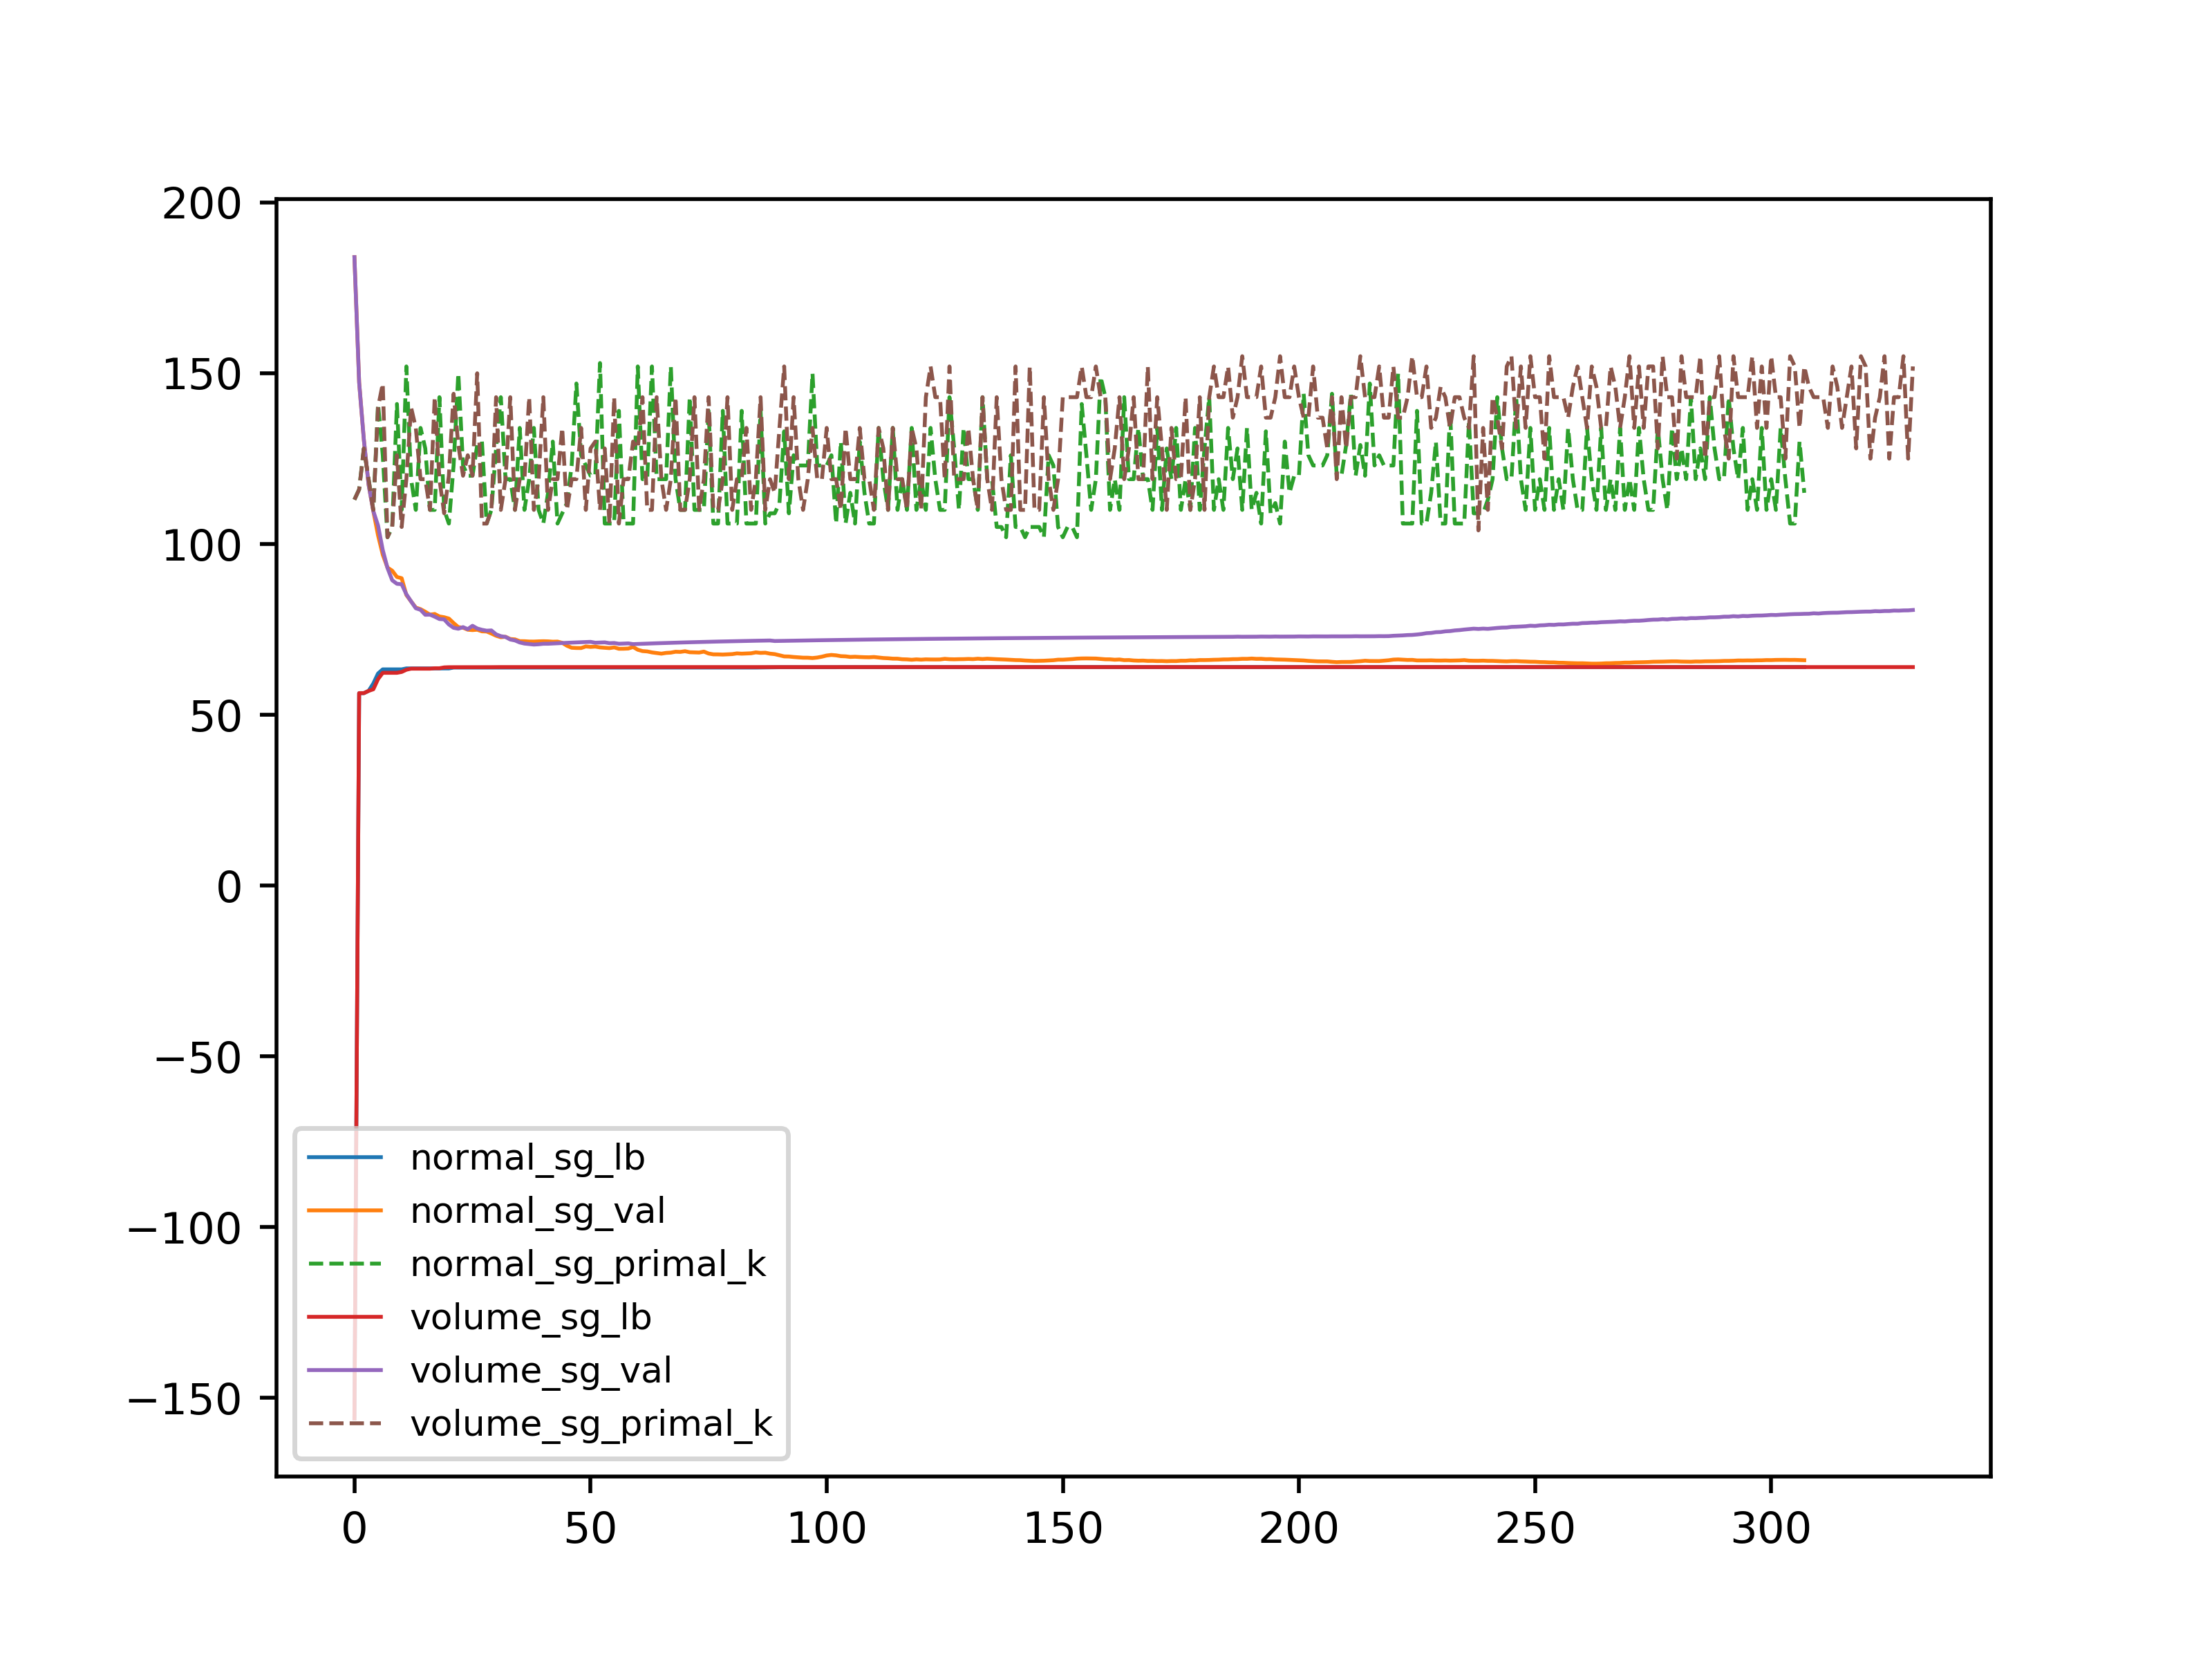
\includegraphics{imgs/conv_0_15_15.png}

\textbf{(So we wish to show the convergence):}
\(|\bar z_k -\hat \phi_k|\)

\hypertarget{reference}{%
  \section*{Reference}\label{reference}}
\addcontentsline{toc}{section}{Reference}

\hypertarget{refs}{}
\begin{CSLReferences}{1}{0}
  \leavevmode\hypertarget{ref-barahona_volume_2000}{}%
  Barahona F, Anbil R (2000) The volume algorithm: Producing primal
  solutions with a subgradient method. \emph{Mathematical Programming}
  87(3):385--399.

  \leavevmode\hypertarget{ref-bertsekas_nonlinear_2016}{}%
  Bertsekas DP (2016) \emph{Nonlinear programming} 3rd ed. (Athena
  Scientific).

  \leavevmode\hypertarget{ref-brannlund1995generalized}{}%
  Brännlund U (1995) A generalized subgradient method with relaxation
  step. \emph{Mathematical Programming} 71(2):207--219.

  \leavevmode\hypertarget{ref-camerini1975improving}{}%
  Camerini PM, Fratta L, Maffioli F (1975) On improving relaxation methods
  by modified gradient techniques. \emph{Nondifferentiable optimization}.
  (Springer), 26--34.

  \leavevmode\hypertarget{ref-kiwiel_lagrangian_2007}{}%
  Kiwiel KC, Larsson T, Lindberg PO (2007) Lagrangian relaxation via
  ballstep subgradient methods. \emph{Mathematics of Operations Research}
  32(3):669--686.

  \leavevmode\hypertarget{ref-nedic_approximate_2009}{}%
  Nedić A, Ozdaglar A (2009) Approximate primal solutions and rate
  analysis for dual subgradient methods. \emph{SIAM Journal on
    Optimization} 19(4):1757--1780.

  \leavevmode\hypertarget{ref-polyak_general_1967}{}%
  Polyak BT (1967) A general method for solving extremal problems.
  \emph{Soviet Mathematics Doklady}:5.

\end{CSLReferences}

\end{document}
